\section{Replacements of pixels.}
\begin{enumerate}[label=\emph{\alph*)}]
\item Take the center square region of 100 x 100 pixels of A and insert it into the center of B.
\begin{figure}[h!]
\centering
\begin{subfigure}{0.5\textwidth}
  \centering
  
\includegraphics[width=0.5\linewidth]{../output/p0-3-a-0.jpg}
  \caption{Output for the input p0-1-0.jpg}
  \label{fig:sfig1}
\end{subfigure}%
\begin{subfigure}{0.5\textwidth}
  \centering
  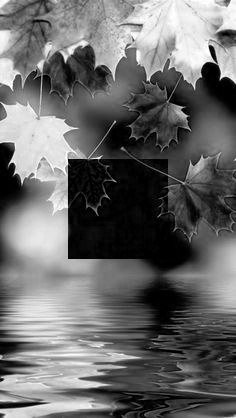
\includegraphics[width=0.5\linewidth]{../output/p0-3-a-1.jpg}
  \caption{Output for the input p0-1-1.jpg}
  \label{fig:sfig2}
\end{subfigure}
\begin{subfigure}{0.5\textwidth}
  \centering
  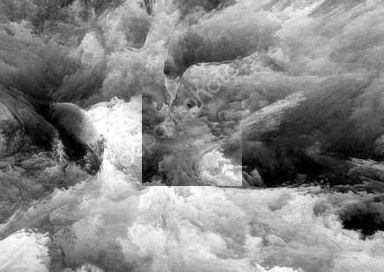
\includegraphics[width=0.5\linewidth]{../output/p0-3-a-2.jpg}
  \caption{Output for the input p0-1-2.jpg}
  \label{fig:sfig1}
\end{subfigure}%
\begin{subfigure}{0.5\textwidth}
  \centering
  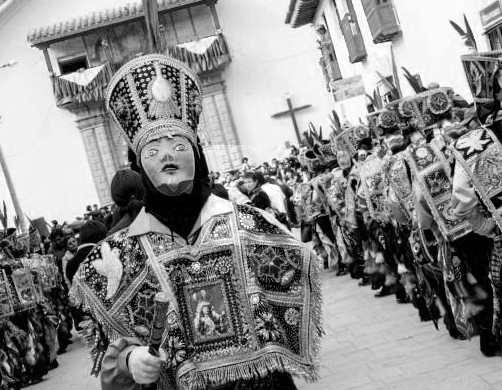
\includegraphics[width=0.5\linewidth]{../output/p0-3-a-3.jpg}
  \caption{Output for the input p0-1-3.jpg}
  \label{fig:sfig2}
\end{subfigure}
\caption{Output images for question 3.a}
\label{fig:fig}
\end{figure}

\item Replace the respective channel of B into the original image
\begin{figure}[h!]
\centering
\begin{subfigure}{0.5\textwidth}
  \centering
  
\includegraphics[width=0.5\linewidth]{../output/p0-3-b-0.jpg}
  \caption{Output for the input p0-1-0.jpg}
  \label{fig:sfig1}
\end{subfigure}%
\begin{subfigure}{0.5\textwidth}
  \centering
  
\includegraphics[width=0.5\linewidth]{../output/p0-3-b-1.jpg}
  \caption{Output for the input p0-1-1.jpg}
  \label{fig:sfig2}
\end{subfigure}
\begin{subfigure}{0.5\textwidth}
  \centering
  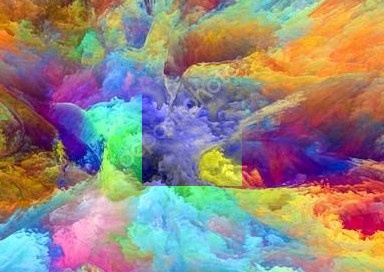
\includegraphics[width=0.5\linewidth]{../output/p0-3-b-2.jpg}
  \caption{Output for the input p0-1-2.jpg}
  \label{fig:sfig1}
\end{subfigure}%
\begin{subfigure}{0.5\textwidth}
  \centering
  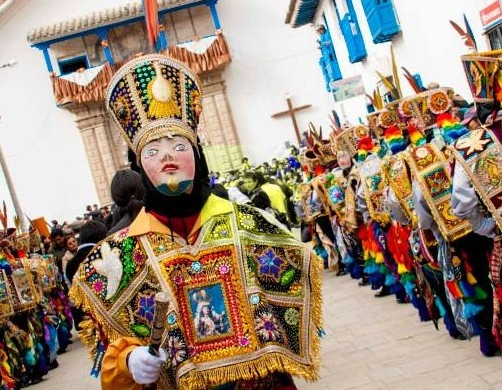
\includegraphics[width=0.5\linewidth]{../output/p0-3-b-3.jpg}
  \caption{Output for the input p0-1-3.jpg}
  \label{fig:sfig2}
\end{subfigure}
\caption{Output images for question 3.b}
\label{fig:fig}
\end{figure}
\\In 3.a the central region of the image B take the values of the central region of the image A. The differences are easily visible.
\\\\In 3.b the output image is the same as the original image, except for the central region, the central region replaced its pixels of the green channel by pixels of the red channel, generating a new color.
\end{enumerate}
